
%\tikzset{every picture/.style={line width=0.75pt}} %set default line width to 0.75pt        



\documentclass[11pt]{beamer}
\usetheme{simple}
\setbeamertemplate{footline}{} 
\usepackage{tikz, pgfplots,amsmath, amssymb, amsthm}   
\usepgfplotslibrary{groupplots}

\usepackage{sansmathaccent}
\pdfmapfile{+sansmathaccent.map}


%\pgfplotsset{ every non boxed y axis/.append style={y axis line style=-}}
\setbeamertemplate{navigation symbols}{}
\begin{document}
\begin{frame}

\only<1>{
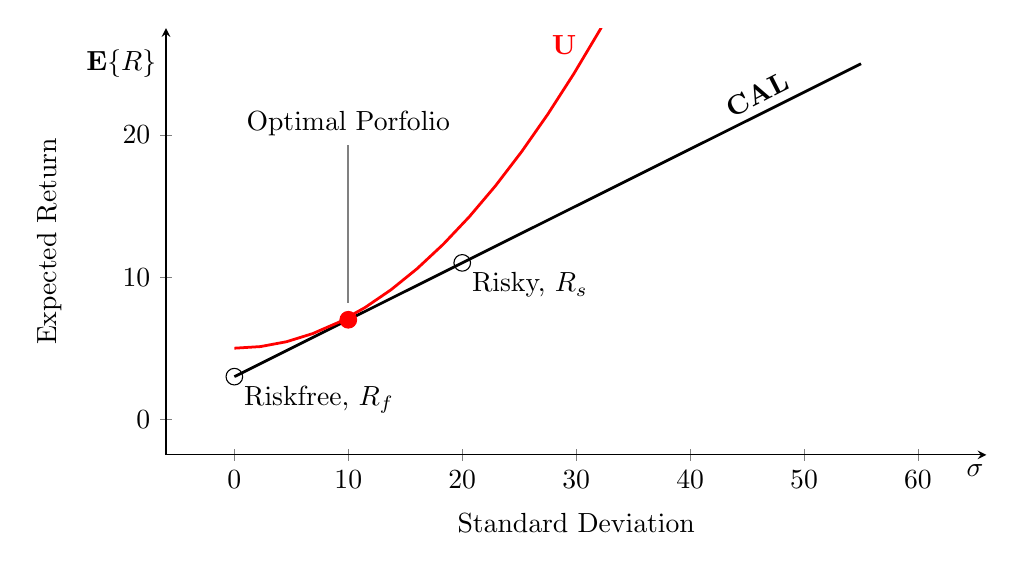
\begin{tikzpicture}[scale=1]
\begin{axis}[
    height=7cm, width=12cm,
    axis x line=bottom, axis y line=left,
    xlabel = Standard Deviation, ylabel = Expected Return,
    ymin=0, ymax=25,
    xmin=0, xmax=60,
    extra x ticks={65}, extra x tick labels={$\sigma$},
    extra x tick style={major tick length=0mm, grid=none},
    extra y ticks={25}, extra y tick labels={$\mathbf{E}\{R\}$},
    extra y tick style={major tick length=0mm, grid=none},
    enlargelimits=true,
    scatter/classes={
      a={mark=o,draw=black, mark size = 3pt},
      b={mark=*, mark size = 3pt,draw=red, fill = red}
    }
]
    \addplot[color=black, domain=0:55, line width=1pt]
      {3 + x * 0.4}; % plot the capital allocation line
    \addplot[color=red, domain=0:55, line width=1pt]
      {5 + 0.5 * (1/23) * x^2}; % plot the utility function
    \addplot[scatter,only marks,
      scatter src=explicit symbolic]  % plot the risk-free rate and the market and the allocation
      coordinates {
          (0,3)        [a]
          (20, 11)     [a]
          (10, 7)      [b]
        };
    \node at (axis cs:0,3) [anchor=north west] {Riskfree, $R_f$};
    \node at (axis cs:20,11) [anchor=north west] {Risky, $R_s$};
    \node[rotate=27] at (axis cs:50, 23) [anchor=south east] {\textbf{CAL}};
    \node[color=red] at (axis cs:27, 25) [anchor=south west] {\textbf{U}};
    \node[pin={[pin edge={thick}, pin distance=2cm]90:{Optimal Porfolio}}] at (axis cs:10,7.5) {};
\end{axis}
\end{tikzpicture}}





\only<2>{
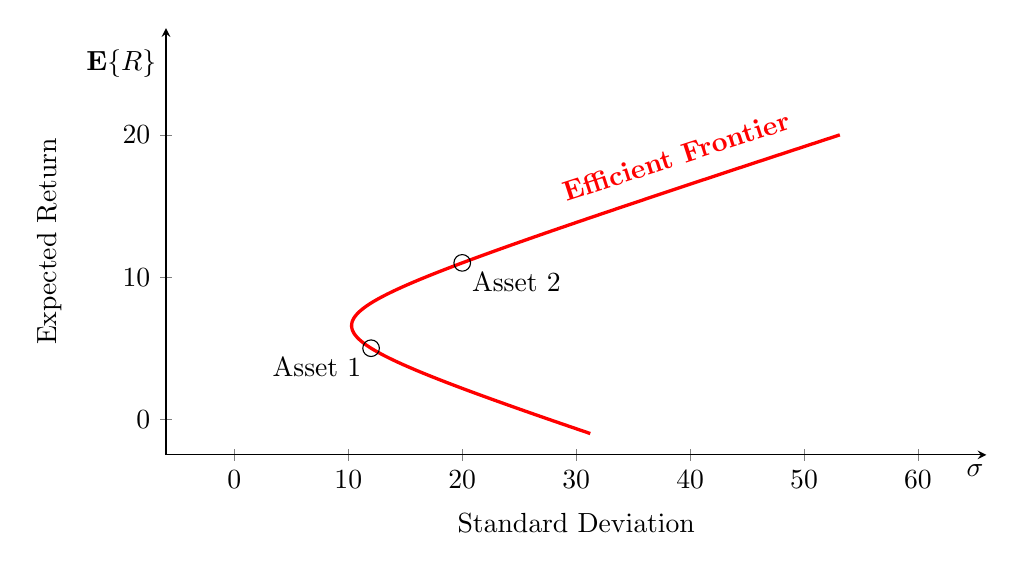
\begin{tikzpicture}
\begin{axis}[
  height=7cm, width=12cm,
  axis x line=bottom, axis y line=left,
  xlabel = Standard Deviation, ylabel = Expected Return,
  ymin=0, ymax=25, xmin=0, xmax=60,
  extra x ticks={65}, extra x tick labels={$\sigma$},
  extra x tick style={major tick length=0mm, grid=none},
  extra y ticks={25}, extra y tick labels={$\mathbf{E}\{R\}$},
  extra y tick style={major tick length=0mm,  grid=none},
  enlargelimits=true,
  scatter/classes={
    a={mark=o,draw=black, mark size = 3pt},
    b={mark=*, mark size = 3pt,draw=red, fill = red}
    }
]

\addplot[scatter,only marks, scatter src=explicit symbolic]
  coordinates {
    (20, 11)     [a]
     (12, 5)      [a]
  };
\node at (axis cs:12, 5) [anchor=north east] {Asset 1};
\node at (axis cs:20,11) [anchor=north west] {Asset 2};
\addplot[red, very thick,  domain=-1:2.5, samples=200, variable=\t](
  {(20^2*t^2 + 12^2*(1-t)^2)^(0.5) }, %{(t^2 * 20^2 + (1-t)^2 * 12)},
  {11 * t + (1-t) * 5} );
\node[rotate=18, color=red] at (axis cs:50, 20) [anchor=south east] {\textbf{Efficient Frontier}};
\end{axis}   
\end{tikzpicture}}





\only<3>{
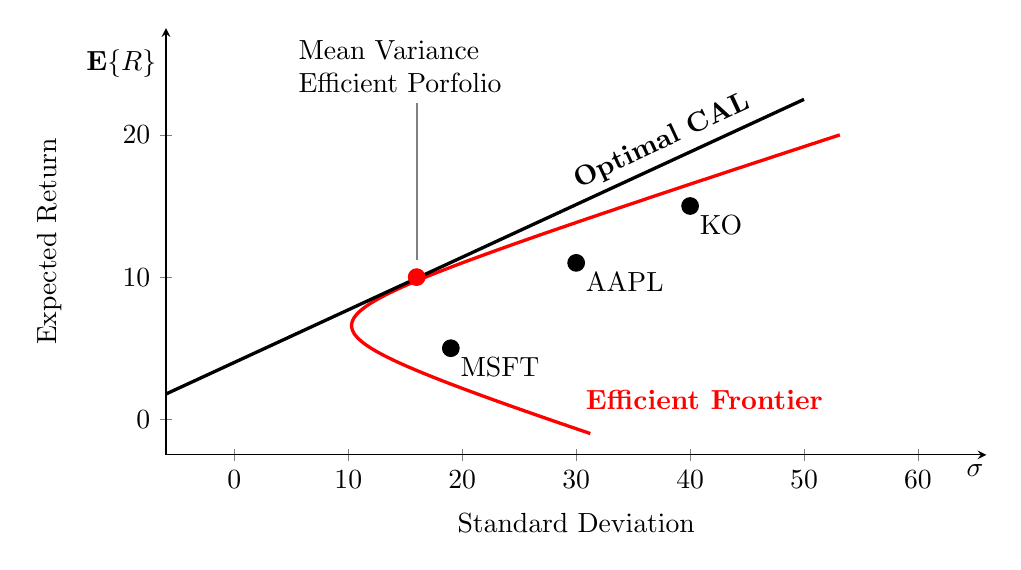
\begin{tikzpicture}
  \begin{axis}[
  height=7cm, width=12cm,
  axis x line=bottom, axis y line=left,
  xlabel = Standard Deviation, ylabel = Expected Return,
  ymin=0, ymax=25, xmin=0, xmax=60,
  extra x ticks={65}, extra x tick labels={$\sigma$},
  extra x tick style={major tick length=0mm, grid=none},
  extra y ticks={25}, extra y tick labels={$\mathbf{E}\{R\}$},
  extra y tick style={major tick length=0mm, grid=none},
  enlargelimits=true,
  scatter/classes={
    a={mark=o,draw=black, mark size = 3pt},
    b={mark=*, mark size = 3pt,draw=red, fill = red},
    c={mark=*, mark size = 3pt,draw=black, fill = black}
  }
]

\addplot[scatter,only marks, scatter src=explicit symbolic]
  coordinates {
    (30, 11)     [c]
    (19, 5)      [c]
    (40, 15)     [c]
    (16, 10)     [b]
  };
\node at (axis cs:19, 5) [anchor=north west] {MSFT};
\node at (axis cs:30,11) [anchor=north west] {AAPL};
\node at (axis cs:40,15) [anchor=north west] {KO};
\addplot[red, very thick,  domain=-1:2.5, samples=200, variable=\t](
   {(20^2*t^2 + 12^2*(1-t)^2)^(0.5) }, %{(t^2 * 20^2 + (1-t)^2 * 12)},
   {11 * t + (1-t) * 5}
 );
\node[color=red] at (axis cs:30, 0) [anchor=south west] {\textbf{Efficient Frontier}};
\addplot[black, very thick, domain=-10:50, samples=100, variable=\x](
  ({x}, {4 + 0.37 * x});
\node[rotate = 25, color=black] at (axis cs:30, 15) [anchor=south west] {\textbf{Optimal CAL}};
\node[pin={[pin edge={thick}, text width=3cm, pin distance=2cm]90:{{\centering Mean Variance Efficient Porfolio}}}] at (axis cs:16, 10.5) {};
\end{axis}
\end{tikzpicture}}






\only<4>{
  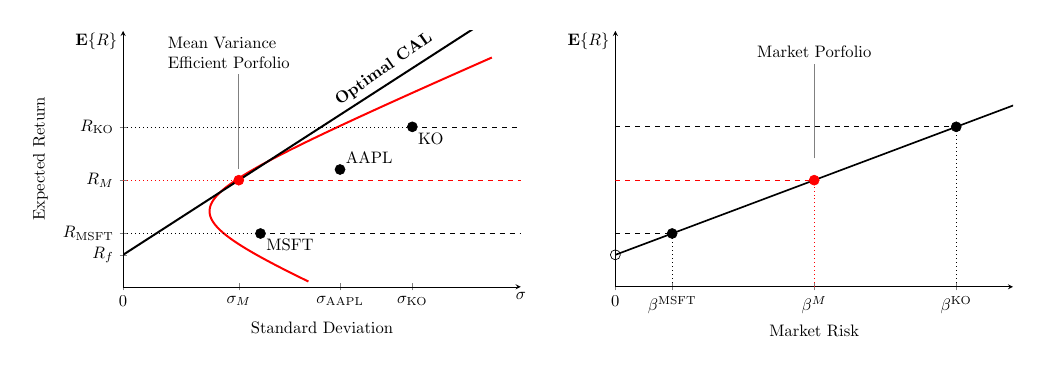
\begin{tikzpicture}[scale=0.6]
    \begin{groupplot}[
      group style={group size=2 by 1, horizontal sep=2cm}, no markers,
      height=7cm, width=10cm,
      axis x line=bottom, axis y line=left,
      ymin=0, ymax=24,
      extra y ticks={23},  extra y tick labels={$\mathbf{E}\{R\}$},
    extra y tick style={major tick length=0mm, grid=none},
    scatter/classes={
      a={mark=o,draw=black, mark size = 3pt},
      b={mark=*, mark size = 3pt,draw=red, fill = red},
      c={mark=*, mark size = 3pt,draw=black, fill = black}
    }
]
% PLOT 1
\nextgroupplot[
    xlabel = Standard Deviation,
    ylabel = Expected Return,
    xmin=0, xmax=55,
    extra x ticks={55}, extra x tick labels={$\sigma$},
    extra x tick style={major tick length=0mm, grid=none},
    xtick={0, 16, 30, 40 },
    xticklabels={0, $\sigma_M$, $\sigma_{\text{AAPL}}$, $\sigma_{\text{KO}}$ },
    ytick={3, 5, 10, 15},
    yticklabels={$R_f$, $R_{\text{MSFT}}$, $R_M$, $R_{\text{KO}}$}
]
    \addplot[scatter,only marks, scatter src=explicit symbolic]
        coordinates {
          (30, 11)     [c]
          (19, 5)      [c]
          (40, 15)     [c]
          (16, 10)     [b]
        };
    \node at (axis cs:19, 5) [anchor=north west] {MSFT};
    \node at (axis cs:30,11) [anchor=south west] {AAPL};
    \node at (axis cs:40,15) [anchor=north west] {KO};
    \addplot[red, very thick,  domain=-0.5:2.5, samples=200, variable=\t](
      {(18^2*t^2 + 16^2*(1-t)^2)^(0.5) }, %{(t^2 * 20^2 + (1-t)^2 * 12)},
      {11 * t + (1-t) * 4}
    );
    \addplot[black, very thick, domain=-10:50, samples=100, variable=\x](({x}, {3 + 7/16 * x});
    \node[rotate = 35, color=black] at (axis cs:30, 16) [anchor=south west]{\textbf{Optimal CAL}};
    \node[pin={[pin edge={thick}, text width=3cm, pin distance=2cm]90:{{\centering Mean Variance Efficient Porfolio}}}] at (axis cs:16, 10.5) {};
    \draw[dotted, color=red] (axis cs:0, 10) -- (axis cs: 16,10);
    \draw[dashed, thick, color=red] (axis cs:16, 10) -- (axis cs: 55,10);
    \node[] (market1) at (axis cs:55.,10) {};
    \draw[dotted] (axis cs:0, 15) -- (axis cs: 40, 15);
    \draw[dashed] (axis cs:40, 15) -- (axis cs: 55,15);
    \node[] (ko1) at (axis cs:55.,15) {};
    \draw[dotted] (axis cs:0, 5) -- (axis cs: 19, 5);
    \draw[dashed] (axis cs:19, 5) -- (axis cs: 55,5);
    \node[] (ms1) at (axis cs:55, 5) {};
  % PLOT 2
  \nextgroupplot[
    xlabel = Market Risk,
    xmin=0, xmax=2,
    xtick={0, 1, 0.2857142857142857, 1.7142857142857142},
    xticklabels={0 , $\beta^M$, $\beta^{\text{MSFT}}$, $\beta^{\text{KO}}$},
    ytick=\empty
  ]
    \addplot[color=black, domain=-10:3, line width=1pt]{3 + x * 7};
    \addplot[scatter,only marks, scatter src=explicit symbolic]
        coordinates {
          (0,3)        [a]
          (1, 10)      [b]
          (2/7, 5)     [c]
          (12/7, 15)   [c]
        };
    \draw[dotted, color=red] (axis cs:1,0) -- (axis cs:1,10);
    \draw[dashed, color=red] (axis cs:0,10) -- (axis cs:1,10);
    \draw[dotted] (axis cs:12/7,0) -- (axis cs:12/7, 15);
    \draw[dashed] (axis cs:0,15) -- (axis cs:12/7,15);
    \draw[dotted] (axis cs:2/7,0) -- (axis cs:2/7, 5);
    \draw[dashed] (axis cs:0,5) -- (axis cs:2/7,5);
    \node[] (market2) at (axis cs:0.,10) {};
    \node[] (ko2) at (axis cs:0,15) {};
    \node[] (ms2) at (axis cs:0, 5) {};
    \node[rotate=23] at (axis cs:2.4, 23) [anchor=south east] {\textbf{SML}};
    \node[pin={[pin edge={thick}, pin distance=2cm]90:{Market Porfolio}}] at (axis cs:1,11.5) {};
  \end{groupplot}
%   \draw[dashed, thick, red] (market1) -- (market2) ;
%   \draw[dashed] (ko1) -- (ko2) ;
%   \draw[dashed] (ms1) -- (ms2) ;
 \end{tikzpicture}}



\end{frame}
\end{document}

\end{tikzpicture}